\documentclass{beamer}
\usetheme{Madrid}
\usepackage{minted}
% sudo tlmgr install minted
\usepackage[utf8]{inputenc}
\usepackage[T2A]{fontenc}
\usepackage[russian,english]{babel}

% Footline: show current section (left) and frame numbers (right)
\setbeamertemplate{footline}{%
  \leavevmode%
  \hbox{%
    \begin{beamercolorbox}[wd=.78\paperwidth,ht=2.5ex,dp=1ex,left]{author in head/foot}%
      \hspace*{1em}\usebeamerfont{footline}\insertsectionhead%
    \end{beamercolorbox}%
    \begin{beamercolorbox}[wd=.22\paperwidth,ht=2.5ex,dp=1ex,right]{date in head/foot}%
      \usebeamerfont{footline}\insertframenumber{} / \inserttotalframenumber\hspace*{1em}%
    \end{beamercolorbox}%
  }%
}

\newcommand{\parpause}[1]{\only<+->{#1\par}}
\newenvironment{definitionbox}[1][Определение]{%
  \begin{exampleblock}{#1}
}{%
  \end{exampleblock}
}

\AtBeginSection[]
{
  \begin{frame}
    \frametitle{Содержание}
    \tableofcontents[currentsection]
  \end{frame}
}

\title{Семинар 5. Репликация, модели согласованности и CAP-теорема}
\subtitle{Распределенные вычисления}
\author{Георгий Семенов}
\institute{Институт прикладных компьютерных наук \\ Университет ИТМО}
\date{весна 2026}

\begin{document}

\frame{\titlepage}

\begin{frame}
\frametitle{Организационные моменты}

\begin{itemize}
  \item Сдвинут DL по первому домашнему заданию – теперь в 23:59 21.03.2026
  \item Второе домашнее задание – жесткий дедлайн в 23:59 02.04.2026
  \begin{itemize}
    \item Полностью с автопроверкой (10 баллов за галочку в GitHub Classroom)
    \item Штраф за сдачу после дедлайна - 50\%
  \end{itemize}
\end{itemize}

\end{frame}

\section{Пессимистическая репликация}

\begin{frame}
\frametitle{Понятие репликации}

\begin{definitionbox}[Репликация]
Избыточное дублирование одного логического объекта на нескольких узлах системы.
\end{definitionbox}

\begin{itemize}
  \item Зачем нужна:
  \begin{itemize}
    \item \textbf{Доступность}: не нужно далеко ходить за данными (данные всегда доступны, даже если другие узлы лежат)
    \item \textbf{Производительность}: параллелизм на чтение, распределение нагрузки
    \item \textbf{Геораспределение}: доступность в плане географических зон
  \end{itemize}
  \item Цена репликации:
  \begin{itemize}
    \item необходимость управлять целостностью данных (integrity)
    \item конфликты и неопределенный порядок событий
  \end{itemize}
\end{itemize}

\end{frame}

\begin{frame}
\frametitle{Две стратегии репликации}

\begin{block}{Стратегия 1: Пессимистическая (синхронная)}
Перед тем как ответить клиенту на запись, синхронизируем со всеми репликами.
\begin{itemize}
  \item Плюс: гарантия что все видят одно и то же
  \item Минус: запись медленна, если упадет какой-то узел — система не отвечает
  \item Разрешение конфликтов a priori
\end{itemize}
\end{block}

\begin{block}{Стратегия 2: Оптимистическая (асинхронная)}
Клиенту ответили сразу, дальше все реплики синхронизируются в фоне.
\begin{itemize}
  \item Плюс: запись быстра, система отвечает даже если узлы падают
  \item Минус: временно разные реплики видят разные значения
  \item Разрешение конфликтов a posteriori
\end{itemize}
\end{block}

\end{frame}

\begin{frame}
\frametitle{Пессимистическая репликация}

\begin{definitionbox}[Пессимистическая репликация]
Синхронная репликация: все изменения синхронизируются \textbf{до} ответа клиенту.
\end{definitionbox}

\begin{itemize}
  \item Почему она называется «пессимистической»?
  \begin{itemize}
    \item Инварианты не могут быть временно нарушены
    \item Баланс счета не должен уйти в минус даже временно
    \item Логин/email должны быть уникальны \textit{сейчас}
    \item Ограничения внешних ключей
  \end{itemize}
  \item Как работает пессимистическая репликация:
  \begin{itemize}
    \item Координатор (мастер) синхронизирует запись со всеми репликами
    \item Используется quorum/consensus: большинство должны подтвердить
    \item Только когда большинство согласны, клиент получает ответ
  \end{itemize}
  \item Типичные механизмы:
  \begin{itemize}
    \item Distributed locks (мьютекствуло между узлами)
    \item Consensus/quorum (Raft, Paxos)
    \item Two-Phase Commit (2PC)
  \end{itemize}
\end{itemize}

\end{frame}

\begin{frame}
\frametitle{Транзакционная модель ACID}

То, какие данные и с какой целью реплицируются, – это детали реализации системы.
Внешняя модель согласованности, свойственная пессимистическим транзакциям, – это ACID: \\

\begin{itemize}
  \item \textbf{Atomicity}: транзакция либо целиком применена, либо откат
  \item \textbf{Consistency}: переход между корректными состояниями БД
  \item \textbf{Isolation}: параллельные транзакции не мешают и не заметны друг другу
  \item \textbf{Durability}: после commit данные переживают сбой узла (WAL)
\end{itemize}

\begin{block}{Важно}
ACID --- это свойства \textit{модели выполнения транзакций}, а не «strong consistency». Но сам подход является пессимистическим.
\end{block}

\end{frame}

\begin{frame}
\frametitle{Linearizability и One-Copy Serializability (1SR)}

\begin{itemize}
  \item \textbf{Linearizability}:
  \begin{itemize}
    \item каждая операция выглядит как мгновенная в момент между invoke/response
    \item если A завершилась раньше, чем B началась, то A должна быть раньше B в глобальном порядке
    \item модель «поведения одной корректной копии в реальном времени»
  \end{itemize}
  \item \textbf{One-Copy Serializability (1SR)}:
  \begin{itemize}
    \item итог эквивалентен некоторому последовательному порядку транзакций над одной копией
    \item не требует сохранения реального времени между независимыми транзакциями
  \end{itemize}
\end{itemize}

\begin{block}{Комментарий}
Linearizability – для атомарных операций записи/чтения, 1SR-Serializability – для транзакций.
\end{block}

\end{frame}

\begin{frame}
\frametitle{Блокировка}

\begin{block}{Понятие блокировки}
Механизм, ограничивающий параллельный доступ к данным для обеспечения их согласованности:
\begin{itemize}
\item \textbf{Shared (S)} --- читать можно многим, писать не может никто
\item \textbf{Exclusive (X)} --- читать и писать может только один
\end{itemize}
\end{block}

\begin{itemize}

  \item Централизованный координатор блокировок
  \begin{itemize}
    \item \textbf{coordinator lock service} (например, ZooKeeper/etcd)
    \item модель check-in/check-out
    \item single point of failure, но может децентрализованным с помощью consensus
  \end{itemize}

  \item Two-Phase Locking (2PL):
  \begin{itemize}
    \item growing phase: только захватываем lock'и
    \item shrinking phase: только освобождаем
  \end{itemize}
  
  \item Риски: deadlocks, high contention (дисциплина обслуживания)
\end{itemize}

\end{frame}

\begin{frame}
\frametitle{Распределенная блокировка}

\begin{block}{Понятие распределенной блокировки}
Блокировка на некоторое время (TTL = Time-to-Live) между узлами в распределенной системе.
\end{block}

\begin{block}{Fencing token}
Монотонно растущий номер владения lock'ом; хранилище обязано отклонять устаревшие токены.
\end{block}

\begin{itemize}
  \item \textbf{lease-based lock} с TTL
  \item Практика: lock + idempotency + timeout + retry с backoff
\end{itemize}

\end{frame}

\begin{frame}
\frametitle{Rate Limiter с помощью распределенной блокировки}

\textbf{Задача:} ограничить количество запросов одного пользователя до N в минуту.

\begin{block}{Наивный подход с глобальной блокировкой}
Для каждого пользователя есть счетчик \texttt{cnt[user]}. При каждом запросе:
\begin{enumerate}
\item захватить \texttt{lock[user]} (прежде чем трогать счетчик)
\item прочитать \texttt{cnt[user]}
\item если \texttt{cnt[user] < N}: инкрементировать, разрешить запрос
\item иначе: отклонить (HTTP 429 Too Many Requests)
\item освободить \texttt{lock[user]}
\end{enumerate}
\end{block}

\end{frame}

\begin{frame}
\frametitle{Optimistic Concurrency Control (OCC)}

Позволяем тразакциям конкурировать, но проверяем их на конфликт в момент commit. Если конфликт — отклоняем одну из транзакций.

\begin{block}{Пример сценария}
Сотрудник Alice и сотрудник Bob редактируют зарплату одного человека.
\begin{itemize}
\item Alice читает: \texttt{salary = 50000}, версия \texttt{v=5}
\item Bob читает: \texttt{salary = 50000}, версия \texttt{v=5}
\item Alice пишет: update to 55000 где \texttt{v=5}
\item Bob пишет: update to 52000 где \texttt{v=5}
\end{itemize}
Из этих двух обновлений только одно может быть принято.
\end{block}

\vspace{0.2cm}

\begin{block}{Увлекательный аспект}\tiny
Техника называется оптимистической, потому что предполагает, что конфликты редки и не стоит блокировать ресурсы заранее.
Но она пессимистическая, потому что в момент commit мы pessimistically проверяем, что никто не изменил данные с момента чтения.
\end{block}

\vspace{0.2cm}

\textbf{Когда хорошо:} много читающих потоков, редкие конфликты, низкая вероятность пересечения на одни и те же данные.

\end{frame}

\section{Оптимистическая репликация}

\begin{frame}
\frametitle{Оптимистическая репликация}

\begin{definitionbox}[Оптимистическая репликация]
Репликация, при которой мы оптимистически разрешаем write-обновления на репликах без предварительной синхронизации.
\end{definitionbox}

\begin{itemize}
  \item Как это работает:
  \begin{itemize}
    \item У каждого узла системы есть своя реплика данных
    \item Чтение и запись производятся с локальной реплики, без синхронизации
    \item Состояния синхронизируются синхронно (gossip, anti-entropy)
  \end{itemize}
  \item Как работать с конфликатми:
  \begin{itemize}
    \item Детерминированно их разрешать без синхронизации (CRDT)
    \item Полуавтоматически и централизованно (семантическая реконсиляция)
    \item Полностью ручной централизованной merge
  \end{itemize}
\end{itemize}

\end{frame}

\begin{frame}
\frametitle{Транзакционная модель BASE}

\begin{itemize}
  \item \textbf{Basically Available}: данные доступны для чтения и записи на узле даже при сбоях других узлов
  \item \textbf{Soft state}: состояние всегда спекулятивное, т.е. мы читаем не «последнее», а «какое-то» значение
  \item \textbf{Eventually consistent}: при отсутствии новых записей реплики сходятся
\end{itemize}

\begin{block}{ACID vs BASE}
ACID оптимизирует корректность синхронного commit, BASE --- доступность и масштаб в условиях partition.
\end{block}

\end{frame}

\begin{frame}
\frametitle{Статья 'Optimistic Replication': M. Shapiro et al. (2005)}

\begin{itemize}
  \item Ввела общий язык для optimistic replication и reconciliation
  \item Ключевые оси классификации:
  \begin{itemize}
    \item state-transfer vs operation-transfer
    \item синхронная vs асинхронная доставка
    \item автоматический vs ручной merge
  \end{itemize}
  \item Главный вывод: нельзя «бесплатно» получить сразу простоту, низкую задержку и сильную согласованность
  \item Практика: проектировать \textbf{типы данных и операции} под возможные конфликты заранее
\end{itemize}
\end{frame}

\begin{frame}
\frametitle{Схема оптимистической репликации}

\begin{center}
    \vspace*{-0.75cm}\hspace*{-2.0cm}
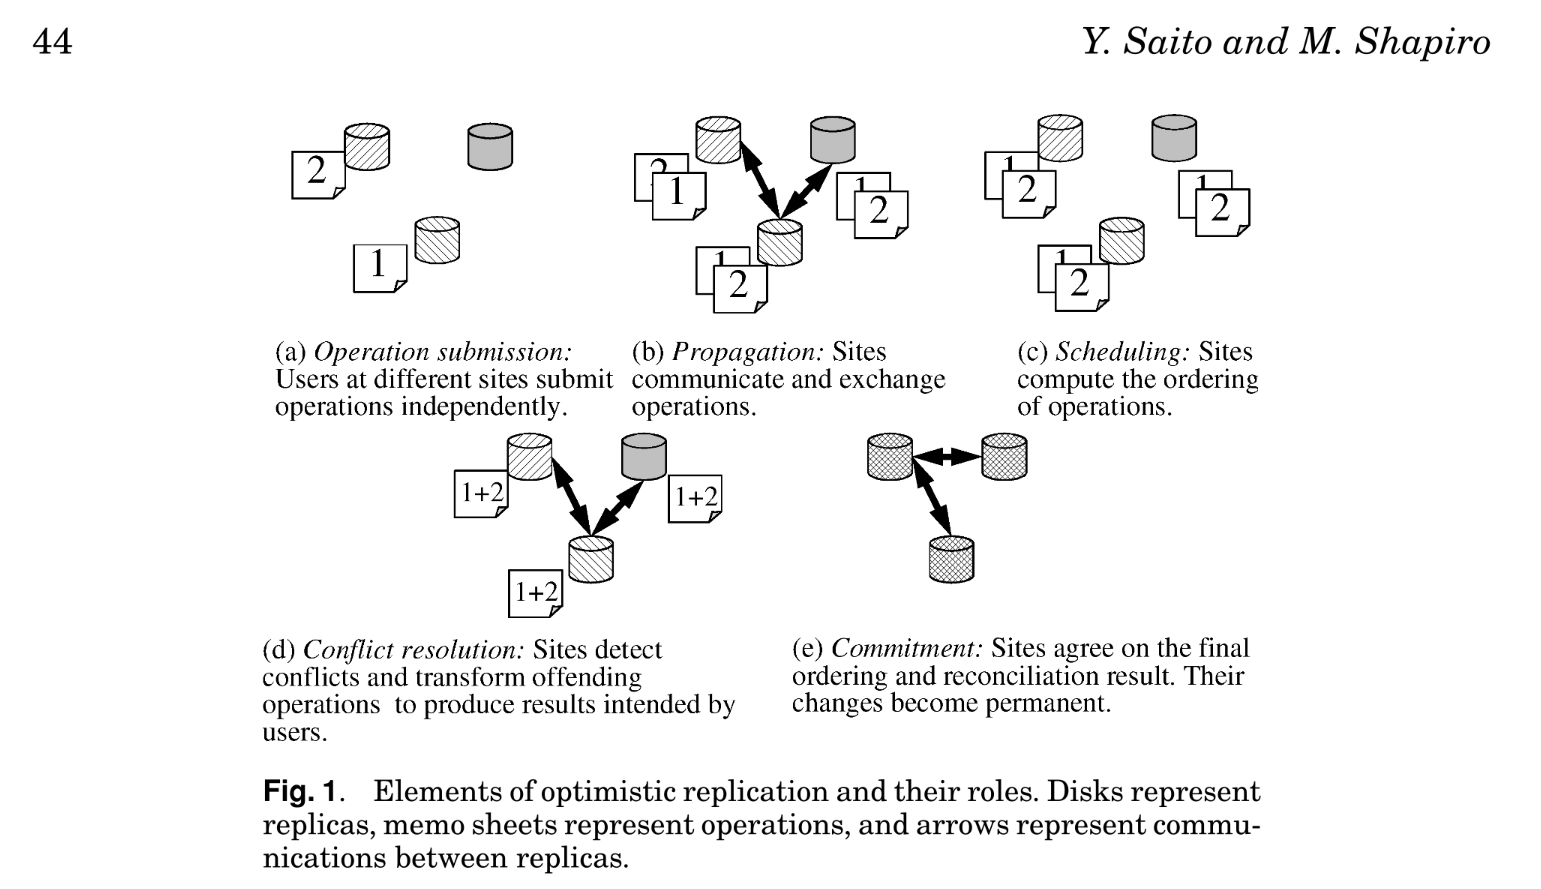
\includegraphics[width=1.25\linewidth,keepaspectratio]{images/shapiro_saito_stages.png}
\end{center}

\end{frame}

\begin{frame}
\frametitle{Знакомые до боли векторные часики}

\begin{center}
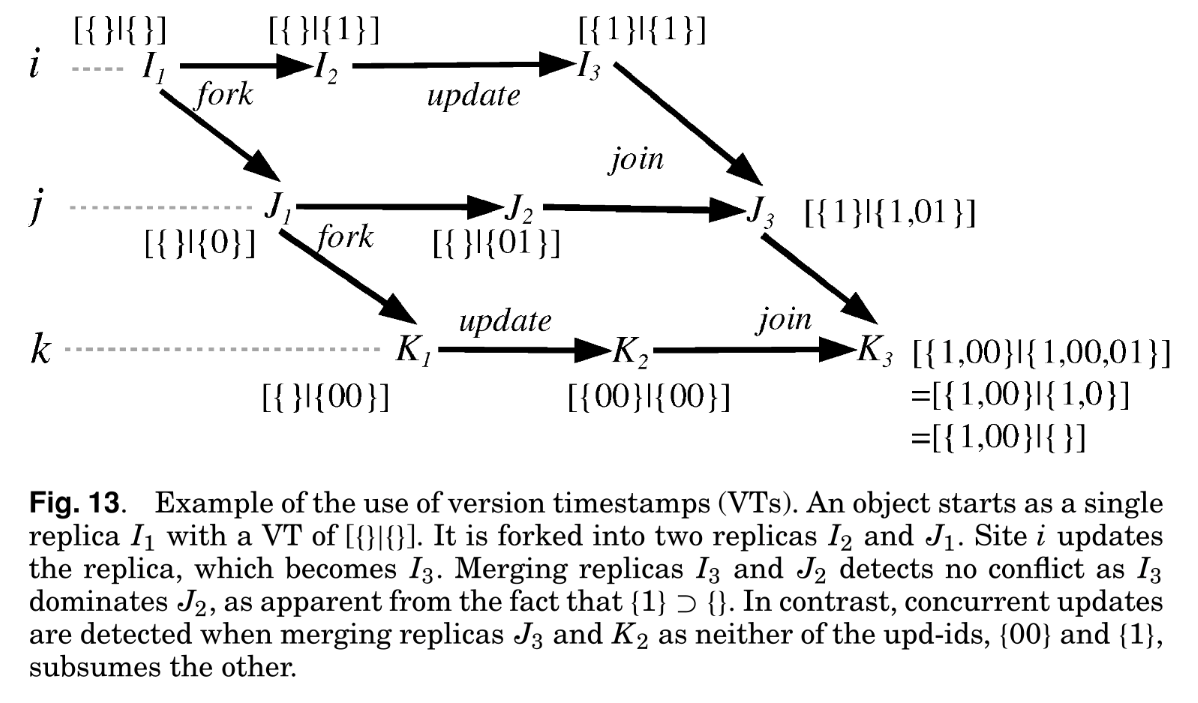
\includegraphics[width=1.0\linewidth,keepaspectratio]{images/shapiro_saito_vector_clocks.png}
\end{center}

\end{frame}

\begin{frame}
\frametitle{Модель Amazon DynamoDB и прикол с корзиной покупок}

\begin{center}
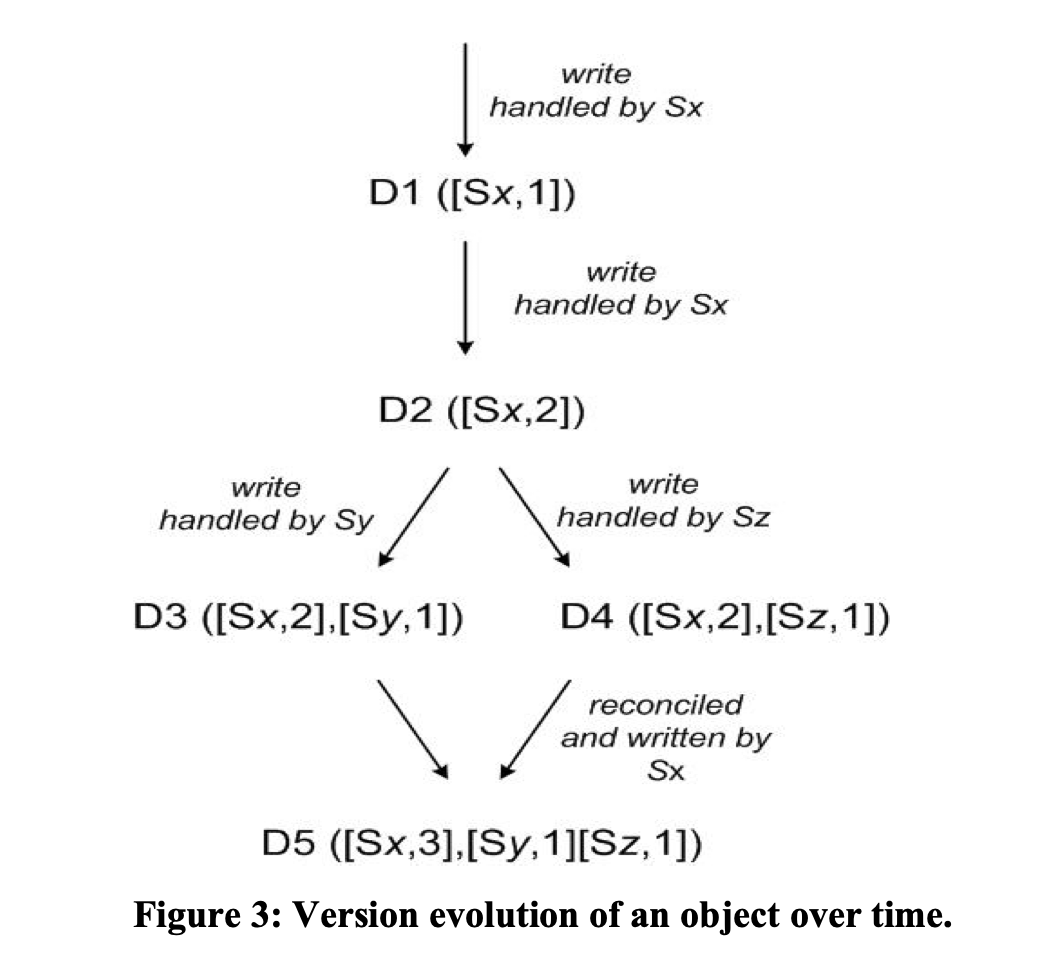
\includegraphics[width=0.7\linewidth,keepaspectratio]{images/dynamodb_mv.png}
\end{center}

\end{frame}

% \begin{frame}
% \frametitle{Анти-энтропийные техники}

% \begin{itemize}
%   \item \textbf{Read repair}: при чтении обнаружили расхождение --- фоново выровняли
%   \item \textbf{Merkle trees}: сравниваем хэши поддеревьев, пересылаем только отличающиеся диапазоны
%   \item \textbf{Gossip протоколы}: узлы периодически обмениваются метаданными о версиях
%   \item \textbf{Hinted handoff}: временно недоступной реплике изменения доставляются позже
% \end{itemize}

% \begin{block}{Цель анти-энтропии}
% Снизить стоимость полного пересканирования и ускорить сходимость реплик.
% \end{block}

% \end{frame}

\section{CAP- и PACELC- теоремы}

\begin{frame}
\frametitle{Почему две стратегии, а не одна?}

\begin{itemize}
  \item Ранее мы увидели два \textbf{противоположных} подхода к репликации
  \item Пессимистический: жертвуем доступностью и задержкой за консистентность
  \item Оптимистический: жертвуем консистентностью за доступность и задержку
\end{itemize}

\begin{block}{Три невозможных желания}
Нельзя одновременно гарантировать:
\begin{itemize}
  \item \textbf{C}onsistency: все видят одно и то же
  \item \textbf{A}vailability: система всегда отвечает
  \item \textbf{P}artition tolerance: система работает когда сеть разломана
\end{itemize}
\end{block}

\end{frame}

\begin{frame}
\frametitle{Необходимые понятия}

\textbf{Network partition} --- когда узлы перестают иметь возможность коммуницировать \\

\begin{itemize}
  \item \textbf{Consistency (C)}: все клиенты видят единое согласованное состояние
  \item \textbf{Availability (A)}: каждый корректный запрос получает ответ
  \item \textbf{Partition tolerance (P)}: система продолжает работу при потере связности между узлами
  \item \textbf{Latency (L)} --- время ответа на запрос
\end{itemize}

\begin{block}{Деталь}
В CAP под C обычно понимают поведение, близкое к linearizability.
\end{block}

\end{frame}

\begin{frame}
\frametitle{CAP-теорема}

\begin{block}{CAP-теорема (Brewer, 2000; Gilbert \& Lynch, 2002)}
В системе нельзя одновременно гарантировать (max 2/3):
\begin{itemize}
  \item \textbf{C}onsistency: сильная согласованность данных
  \item \textbf{A}vailability: доступность
  \item \textbf{P}artition tolerance: устойчивость к сетевым разрывам
\end{itemize}
\end{block}


\end{frame}

\begin{frame}
\frametitle{Детали про CAP-теорему}

\begin{itemize}
  \item \textbf{CP}: отклоняем часть запросов, но не отдаем противоречивые ответы
  \item \textbf{AP}: отвечаем всегда, но допускаем временную рассогласованность
\end{itemize}

\begin{block}{Классы систем}
Любая система относится либо к CP (пессимистическая), либо к AP (оптимистическая).
\end{block}

\begin{alertblock}{Важный момент}
CA-система возможна только если игнорировать partition как класс сбоев, что наивно.
\end{alertblock}

\end{frame}

\begin{frame}
\frametitle{'Critique of CAP theorem' (Kleppmann, 2014)}

\begin{itemize}
  \item Сетевые разрывы – это настолько очевидный тип отказа, что глупо говорить отдельно, что мы можем его игнорировать (P)
  \item По факту выбираем между C и A, при этом упускаем измерение L (latency)
  \item Подход Клеппманна:
  \begin{itemize}
    \item Разделим операции на delay-dependent и delay-independent
    \item Для delay-independent операций можно достичь и C, и A
    \item Иначе выбираем C или A в зависимости от требований к задержке
  \end{itemize}
\end{itemize}

\end{frame}

\begin{frame}
\frametitle{PACELC-теорема}

\begin{itemize}
  \item \textbf{If P} (partition): выбор между \textbf{A} и \textbf{C}
  \item \textbf{Else} (нет partition): выбор между \textbf{L} (latency) и \textbf{C}
  \item Примеры:
  \begin{itemize}
    \item \textbf{PA/EL}: Dynamo-подобные системы (в норме низкая задержка)
    \item \textbf{PC/EC}: системы, жертвующие latency ради строгой согласованности
  \end{itemize}
\end{itemize}

\begin{block}{Инженерный смысл}
Компромисс между скоростью и консистентностью существует всегда, даже когда сеть «здоровая».
\end{block}

\end{frame}

\section{Модели согласованности}

\begin{frame}
\frametitle{Понятие согласованности}

\begin{itemize}
  \item \textbf{Модель согласованности} задает, какие значения при чтении система может вернуть после записей
  \item Это контракт между клиентским кодом и хранилищем
  \item Чем слабее модель, тем проще масштабироваться и выше доступность
  \item Чем сильнее модель, тем меньше аномалий, но выше задержка
\end{itemize}

\end{frame}

\begin{frame}
\frametitle{Consistency vs. Integrity}

\begin{columns}
\column{0.5\textwidth}
\textbf{Consistency (видимость)}
\begin{itemize}
  \item Какие допустимые состояния системы видны нам после изменения
  \item Должны ли мы видеть обновление? С какой допустимой задержкой? В каком порядке?
  \item Пример: read-your-writes (session consistency)
\end{itemize}

\column{0.5\textwidth}
\textbf{Integrity (инварианты)}
\begin{itemize}
  \item Какие состояния запрещены
  \item Пример: \texttt{balance >= 0}, уникальность email
\end{itemize}
\end{columns}

\vspace{0.3cm}
\begin{alertblock}{Это два параллельных измерения}
Можно иметь strong consistency и при этом нарушать integrity из-за неверной бизнес-логики.
\end{alertblock}

\end{frame}

\begin{frame}
\frametitle{Некоторые важные модели по M. Perrin}

\begin{columns}
    \column{0.5\textwidth}
        \begin{center}
            \vspace*{-1cm}
            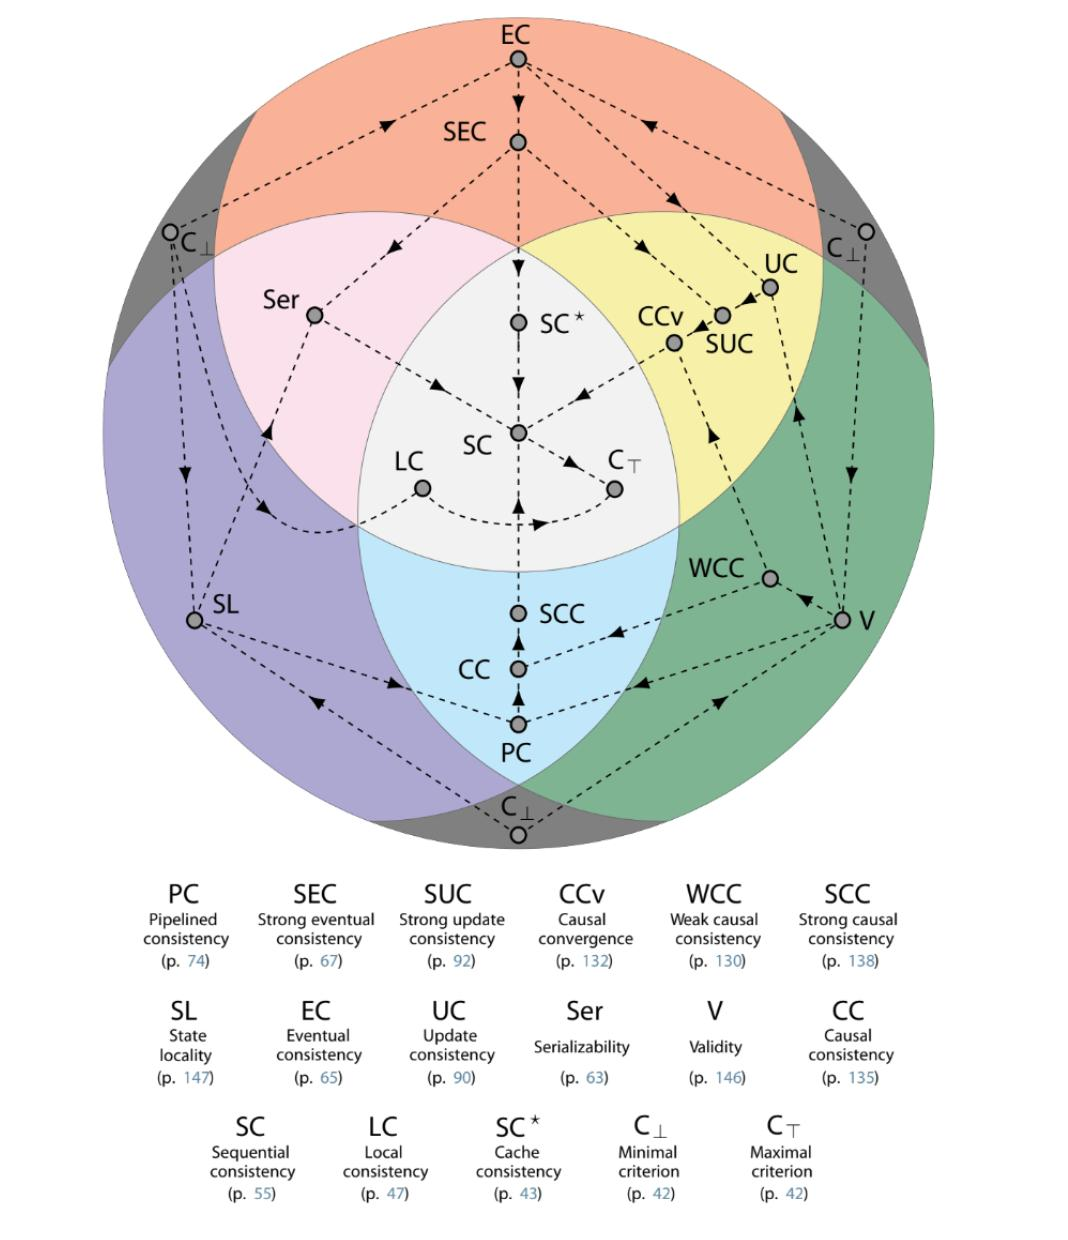
\includegraphics[width=1.1\linewidth,keepaspectratio]{images/perrin_consistencies.png}
        \end{center}
        
        \column{0.5\textwidth}
        \begin{enumerate}
            \item \textbf{Strong Consistency} \\
            Все операции читают последнее записанное значение
            
            \item \textbf{Sequential Consistency} \\
            Существует общий линейный порядок операций
            
            \item \textbf{Causal Consistency} \\
            Happens-before порядок сохраняется
            
            \item \textbf{Eventual Consistency} \\
            Спустя какое-то время реплики сойдутся

            \item \textbf{Strong Eventual Consistency} \\
            Реплика = множество полученных ей сообщений
        \end{enumerate}
\end{columns}

\end{frame}

\begin{frame}
\frametitle{Strong Consistency}

\begin{itemize}
  \item Любое чтение возвращает результат последней завершенной записи
  \item Поведение эквивалентно «одной копии» данных
  \item Плюсы: простой mental model для разработчика
  \item Минусы: выше latency (часто нужен кворум/лидер), чувствительность к partition
\end{itemize}

\textbf{Подходит:} платежи, инвентарь, дедупликация критичных операций.

\end{frame}

\begin{frame}
\frametitle{Sequential Consistency}

\begin{itemize}
  \item Все операции наблюдаются в одном и том же \textbf{глобальном порядке}
  \item Этот порядок согласован с \textbf{порядком операций каждого отдельного клиента}
  \item Но не обязан совпадать с реальным временем
\end{itemize}

\begin{block}{Следствие}
Операция, завершившаяся раньше по wall-clock, может оказаться позже в глобальном порядке.
\end{block}

\end{frame}

\begin{frame}
\frametitle{Strong vs. Sequential Consistency}

\begin{center}
\begin{tabular}{p{0.5\linewidth}p{0.25\linewidth}p{0.25\linewidth}}
\textbf{Свойство} & \textbf{Strong} & \textbf{Sequential} \\ \hline
Единый порядок операций & Да & Да \\
Учет реального времени & Да & Нет \\
Влияние сетевых задержек & Выше & Ниже \\
\end{tabular}
\end{center}

\vspace{0.2cm}
\textbf{Грубо говоря:} strong = sequential + real-time constraints.

\end{frame}

\begin{frame}
\frametitle{Семейство моделей Weak Consistency}

\begin{itemize}
  \item Не гарантируют единого «актуального» значения в каждый момент
  \item Часто дают локальные гарантии:
  \begin{itemize}
    \item Read Your Writes
    \item Monotonic Reads
    \item Monotonic Writes
    \item Writes Follow Reads
  \end{itemize}
  \item Идея: выбрать \textbf{минимально достаточную} гарантию под конкретный use-case
\end{itemize}

\end{frame}

\begin{frame}
\frametitle{Eventual Consistency}

\begin{itemize}
  \item Если новые записи прекратились, все реплики в итоге сходятся
  \item Не гарантирует срок сходимости
  \item На практике требуется:
  \begin{itemize}
    \item анти-энтропия
    \item детерминированный merge
    \item контроль clock skew (для LWW)
  \end{itemize}
\end{itemize}

\textbf{Типичный сценарий:} кеши, каталоги, ленты рекомендаций.

\end{frame}

\begin{frame}
\frametitle{Causal Consistency}

\begin{itemize}
  \item Сохраняет отношение happens-before между причинно связанными операциями
  \item Конкурентные (независимые) записи могут наблюдаться в разном порядке
  \item Пример:
  \begin{itemize}
    \item пользователь A публикует пост
    \item пользователь B отвечает на пост
    \item нельзя увидеть ответ, не увидев исходный пост
  \end{itemize}
\end{itemize}

\textbf{Механизмы:} vector clocks, dependency tracking.

\end{frame}

\begin{frame}
\frametitle{Strong Eventual Consistency}

\begin{itemize}
  \item При доставке одного и того же набора обновлений все реплики гарантированно равны
  \item Порядок доставки не важен
  \item Обычно достигается через CRDT:
  \begin{itemize}
    \item операции коммутативны
    \item merge ассоциативен, коммутативен и идемпотентен
  \end{itemize}
\end{itemize}

\textbf{Примеры:} счетчики, множества, совместное редактирование документов.

\end{frame}

\begin{frame}
\frametitle{Session Consistency}

\begin{itemize}
  \item Гарантии только внутри одной клиентской сессии
  \item Наиболее полезные свойства:
  \begin{itemize}
    \item Read Your Writes
    \item Monotonic Reads
  \end{itemize}
  \item После реконнекта к другому региону гарантия может временно пропасть
  \item Практика: sticky sessions или session token с версией
\end{itemize}

\end{frame}

\begin{frame}
\frametitle{Как выбирать модель согласованности на практике}

\begin{enumerate}
  \item Выписать бизнес-инварианты (что \textbf{никогда} нельзя нарушить)
  \item Разделить операции на критичные и некритичные
  \item Назначить минимальную достаточную модель на операцию
  \begin{itemize}
    \item платеж/списание: strong или serializable транзакции
    \item лента/счетчики просмотров: eventual или causal
    \item профиль пользователя: session guarantees часто достаточно
  \end{itemize}
  \item Контролировать production через p95/p99 latency и частоту конфликтов
\end{enumerate}

\end{frame}


% \section{Синхронные и асинхронные распределенные системы}

% \begin{frame}
% \frametitle{}

% \begin{itemize}
   
% \end{itemize}

% \end{frame}

% \section{FLP-теорема}

% \begin{frame}
% \frametitle{}

% \begin{itemize}
   
% \end{itemize}

% \end{frame}

\begin{frame}
\frametitle{Итоги}

\begin{itemize}
  \item (!) Выдано второе домашнее задание
  \item Обсудили понятие репликации и две противоположные стратегии: пессимистическую и оптимистическую
  \item CAP-теорема иллюстрирует, почему важны и нужны оба подхода
  \item Разные модели согласованности – разные гарантии видимости данных
\end{itemize}

\end{frame}

\end{document}